\documentclass[11pt,openany]{article}

\usepackage{mathtools, commath}
% Packages for formatting
\usepackage[margin=1in]{geometry}
\usepackage{fancyhdr}
\usepackage{enumerate}
\usepackage{graphicx}
\usepackage{kotex}
\usepackage{arydshln} % Include this package
\usepackage{bbding}
\usepackage{amsmath}
\usepackage{amsthm}
\usepackage[dvipsnames,table]{xcolor}
\usepackage{amssymb, amsfonts}
\usepackage{wasysym}
\usepackage{footnote}
\usepackage{tablefootnote}
\usepackage{arydshln} % Include this package
% Fonts
\usepackage[T1]{fontenc}
\usepackage[utf8]{inputenc}
\usepackage{newpxtext,newpxmath}
\usepackage{sectsty}

% Define colors
\definecolor{TealBlue1}{HTML}{0077c2}
\definecolor{TealBlue2}{HTML}{00a5e6}
\definecolor{TealBlue3}{HTML}{b3e0ff}
\definecolor{TealBlue4}{HTML}{00293c}
\definecolor{TealBlue5}{HTML}{e6f7ff}

\definecolor{thmcolor}{RGB}{231, 76, 60}
\definecolor{defcolor}{RGB}{52, 152, 219}
\definecolor{lemcolor}{RGB}{155, 89, 182}
\definecolor{corcolor}{RGB}{46, 204, 113}
\definecolor{procolor}{RGB}{241, 196, 15}

\usepackage{color,soul}
\usepackage{soul}
\newcommand{\mathcolorbox}[2]{\colorbox{#1}{$\displaystyle #2$}}
\usepackage{cancel}
\newcommand\crossout[3][black]{\renewcommand\CancelColor{\color{#1}}\cancelto{#2}{#3}}
\newcommand\ncrossout[2][black]{\renewcommand\CancelColor{\color{#1}}\cancel{#2}}

\usepackage{hyperref}
\usepackage{booktabs}

% Chapter formatting
\definecolor{titleTealBlue}{RGB}{0,53,128}
\usepackage{titlesec}
\titleformat{\section}
{\normalfont\sffamily\Large\bfseries\color{titleTealBlue!100!gray}}{\thesection}{1em}{}
\titleformat{\subsection}
{\normalfont\sffamily\large\bfseries\color{titleTealBlue!50!gray}}{\thesubsection}{1em}{}

%Tcolorbox
\usepackage[most]{tcolorbox}
\usepackage{multirow}
\usepackage{multicol}
\usepackage{blindtext}

\usepackage[linesnumbered,ruled]{algorithm2e}
\usepackage{algpseudocode}
\usepackage{setspace}
\SetKwComment{Comment}{/* }{ */}
\SetKwProg{Fn}{Function}{:}{end}
\SetKw{End}{end}
\SetKw{DownTo}{downto}

% Define a new environment for algorithms without line numbers
\newenvironment{algorithm2}[1][]{
	% Save the current state of the algorithm counter
	\newcounter{tempCounter}
	\setcounter{tempCounter}{\value{algocf}}
	% redefine the algorithm numbering (remove prefix)
	\renewcommand{\thealgocf}{}
	\begin{algorithm}
	}{
	\end{algorithm}
	% Restore the algorithm counter state
	\setcounter{algocf}{\value{tempCounter}}
}

\usepackage{adjustbox}
% Header and footer formatting
\pagestyle{fancy}
\fancyhead{}
\fancyhf{}
\rhead{\textcolor{TealBlue2}{\large\textbf{기대수(기초부터 대학원 수학까지 시리즈) 3기}}}%\rule{3cm}{0.4pt}}
\lhead{\textcolor{TealBlue2}{\large\textbf{수학의 즐거움, Enjoying Math}}}
% Define footer
%\newcommand{\footer}[1]{
%\begin{flushright}
%	\vspace{2em}
%	\includegraphics[width=2.5cm]{school_logo.jpg} \\
%	\vspace{1em}
%	\textcolor{TealBlue2}{\small\textbf{#1}}
%\end{flushright}
%}
%\rfoot{\large Department of Information Security, Cryptogrphy and Mathematics, Kookmin Uni.\includegraphics[height=1.5cm]{school_logo.jpg}}
\fancyfoot{}
\fancyfoot[C]{-\thepage-}

\usepackage{tcolorbox}
\tcbset{colback=white, arc=5pt}

\definecolor{axiomcolor}{HTML}{a88bfa}
\definecolor{defcolor}{RGB}{52, 152, 219}
\definecolor{procolor}{RGB}{241, 196, 15}
\definecolor{thmcolor}{RGB}{231, 76, 60}
\definecolor{lemcolor}{RGB}{155, 89, 182}
\definecolor{corcolor}{RGB}{46, 204, 113}
\definecolor{execolor}{RGB}{90, 128, 127}

% Define a new command for the custom tcolorbox
\newcommand{\axiombox}[2][]{%
	\begin{tcolorbox}[colframe=axiomcolor, title={\color{white}\bfseries #1}]
		#2
	\end{tcolorbox}
}

\newcommand{\defbox}[2][]{%
	\begin{tcolorbox}[colframe=defcolor, title={\color{white}\bfseries #1}]
		#2
	\end{tcolorbox}
}

\newcommand{\lembox}[2][]{%
	\begin{tcolorbox}[colframe=lemcolor, title={\color{white}\bfseries #1}]
		#2
	\end{tcolorbox}
}

\newcommand{\probox}[2][]{%
	\begin{tcolorbox}[colframe=procolor, title={\color{white}\bfseries #1}]
		#2
	\end{tcolorbox}
}

\newcommand{\thmbox}[2][]{%
	\begin{tcolorbox}[colframe=thmcolor, title={\color{white}\bfseries #1}]
		#2
	\end{tcolorbox}
}

\newcommand{\corbox}[2][]{%
	\begin{tcolorbox}[colframe=corcolor, title={\color{white}\bfseries #1}]
		#2
	\end{tcolorbox}
}



\usepackage{amsthm}

% Define custom theorem styles
\newtheoremstyle{dotless} % Name of the style
{3pt} % Space above
{3pt} % Space below
{\itshape} % Body font
{} % Indent amount
{\bfseries} % Theorem head font
{} % Punctuation after theorem head
{2.5mm} % Space after theorem head
{} % Theorem head spec

\newtheoremstyle{definitionstyle} % Name of the style
{3pt} % Space above
{3pt} % Space below
{} % Body font
{} % Indent amount
{\bfseries} % Theorem head font
{.} % Punctuation after theorem head
{2.5mm} % Space after theorem head
{} % Theorem head spec

% Applying custom styles
\theoremstyle{dotless}
\newtheorem{theorem}{Theorem} % Theorem environment with section-wise numbering
\newtheorem{proposition}[theorem]{Proposition} % Theorem environment with section-wise numbering
\newtheorem{lemma}[theorem]{Lemma} % Lemma shares the counter with theorem
\newtheorem{corollary}[theorem]{Corollary} % Corollary shares the counter with theorem

\theoremstyle{definitionstyle}
\newtheorem*{observation}{\textcolor{Magenta}{Observation}}
\newtheorem{definition}{Definition} % Definition shares the counter with theorem
\newtheorem{example}{Example} % Example shares the counter with theorem
\newtheorem{exercise}{Exercise} % Example shares the counter with theorem
\newtheorem{remark}{Remark} % Remark shares the counter with theorem
\newtheorem*{note}{Note}

\newtheorem*{definition*}{Definition} % Definition shares the counter with theorem
\newtheorem*{example*}{Example} % Example shares the counter with theorem
\newtheorem*{exercise*}{\textcolor{violet}{Exercise}} % Example shares the counter with theorem
\newtheorem*{remark*}{Remark} % Remark shares the counter with theorem


\usepackage{tikz}
\usepackage{tikz-cd}
\usepackage{tikz-3dplot}
\usepackage{pgfplots}
\pgfplotsset{compat=newest} % Adjust to your version of pgfplots
\def\Circlearrowleft{\ensuremath{%
		\rotatebox[origin=c]{180}{$\circlearrowleft$}}}
\def\Circlearrowright{\ensuremath{%
		\rotatebox[origin=c]{180}{$\circlearrowright$}}}
\def\CircleArrowleft{\ensuremath{%
		\reflectbox{\rotatebox[origin=c]{180}{$\circlearrowleft$}}}}
\def\CircleArrowright{\ensuremath{%
		\reflectbox{\rotatebox[origin=c]{180}{$\circlearrowright$}}}}
\usetikzlibrary{
	3d, % For 3D drawing
	angles,
	arrows,
	arrows.meta,
	backgrounds,
	bending,
	calc,
	decorations.pathmorphing,
	decorations.pathreplacing,
	decorations.markings,
	fit,
	matrix,
	patterns,
	patterns.meta,
	positioning,
	quotes,
	shadows,
	shapes,
	shapes.geometric,
	tikzmark
}
\tikzset{
	% single mid‐path arrow
	mid arrow/.style={
		decoration={
			markings,
			mark=at position 0.5 with {\arrow{Stealth[scale=1.2]}}
		},
		postaction={decorate},
	},
	% style for field arrows
	field arrow/.style={
		-{Stealth[scale=1.0]},
		thick,
		blue!70!black,
	},
}
\newcommand{\ie}{\textnormal{i.e.}}
\newcommand{\rsa}{\mathsf{RSA}}
\newcommand{\rsacrt}{\mathsf{RSA}\textendash\mathsf{CRT}}
\newcommand{\inv}[1]{#1^{-1}}

%New Command
%\newcommand{\set}[1]{\left\{#1\right\}}
\newcommand{\N}{\mathbb{N}}
\newcommand{\Z}{\mathbb{Z}}
\newcommand{\Q}{\mathbb{Q}}
\newcommand{\R}{\mathbb{R}}
\newcommand{\cR}{\mathcal{R}}
\newcommand{\C}{\mathbb{C}}
\newcommand{\F}{\mathbb{F}}
\newcommand{\nbhd}{\mathcal{N}}
\newcommand{\Log}{\operatorname{Log}}
\newcommand{\Arg}{\operatorname{Arg}}
\newcommand{\pv}{\operatorname{P.V.}}

\newcommand{\of}[1]{\left( #1 \right)} 
%\newcommand{\abs}[1]{\left\lvert #1 \right\rvert}
%\newcommand{\norm}[1]{\left\| #1 \right\|}

\newcommand{\sol}{\textcolor{magenta}{\bf Sol}}
\newcommand{\conjugate}[1]{\overline{#1}}

\newcommand{\res}{\operatorname{res}}
\DeclareMathOperator*{\Res}{\operatorname{Res}}

%\renewcommand{\Re}{\operatorname{Re}}
%\renewcommand{\Im}{\operatorname{Im}}

\newcommand{\cyclic}[1]{\langle #1 \rangle}
\newcommand{\uniform}{\overset{\$}{\leftarrow}}
\newcommand{\xmark}{\textcolor{red}{\XSolidBrush}}
\newcommand{\vmark}{\textcolor{green!75!black}{\CheckmarkBold}}

\newcommand{\gen}[1]{\langle #1 \rangle}
\newcommand{\Gen}[1]{\left\langle #1 \right\rangle}

\newcommand{\img}[1]{\text{Img}(#1)}
\newcommand{\Img}[1]{\text{Img}\left(#1\right)}
\newcommand{\preimg}[1]{\text{Img}^{-1}(#1)}
\newcommand{\Preimg}[1]{\text{Img}^{-1}\left(#1\right)}

\newcommand{\relation}{\mathrel{\mathcal{R}}}
\newcommand{\injection}{\rightarrowtail}
\newcommand{\surjection}{\twoheadrightarrow}
\newcommand{\id}{\textnormal{id}}

\newcommand{\eqclass}[1]{\left[#1\right]}

% Define custom colors for O and X
\newcommand{\yes}{\textcolor{blue}{\bf \fullmoon}}
\newcommand{\no}{\textcolor{red}{\bf \texttimes}}

\DeclarePairedDelimiter\ceil{\lceil}{\rceil}
\DeclarePairedDelimiter\floor{\lfloor}{\rfloor}
%\renewcommand{\floor}[#1]{\lfloor #1\rfloor}
%\newcommand{\Floor}[#1]{\left\lfloor #1\right\rfloor}
%\newcommand{\ceil}[#1]{\lceil #1\rceil}
%\newcommand{\Ceil}[#1]{\left\lceil #1\right\rceil}

\newcommand{\topology}{\mathscr{T}}
\newcommand{\sequence}[1]{\langle #1\rangle}

% Topology
%\newcommand{\nbhd}{\mathcal{N}}

% Linear Algebra
\newcommand{\Span}{\operatorname{\normalfont span}}
\newcommand{\basis}{\mathcal{B}}
\newcommand{\card}[1]{\text{\normalfont card}(#1)}
\renewcommand{\vec}[1]{\mathbf{#1}}
\renewcommand{\Re}{\operatorname*{Re}}
\renewcommand{\Im}{\operatorname*{Im}}
\setstretch{1.25}

%\usepackage{background}
%\backgroundsetup{
%	scale=3,
%	color=gray!20,
%	opacity=0.3,
%	angle=45,
%	contents={\Huge \sffamily Ji, Yong-hyeon}
%}
\begin{document}
\pagenumbering{arabic}
\begin{center}
	\huge\textbf{{\color{red}T}{\color{orange}o}{\color{green!75!black}r}{\color{cyan}u}{\color{violet}s} and Algebra}\\
	\vspace{0.5em}
	\large{Ji, Yong-hyeon}\\
%	\large{\ttfamily \url{https://github.com/Hacker-Code-J}}\\
	\vspace{0.5em}
	\normalsize{\today}\\
\end{center}

\noindent 
We cover the following topics in this note.
\begin{itemize}
	\item Unit Circle
	\item {\bfseries\color{red}T}{\color{orange}o}{\color{green!75!black}r}{\color{cyan}u}{\color{violet}s}
	\item TBA
\end{itemize}
\hrule\vspace{12pt}
\begin{center}
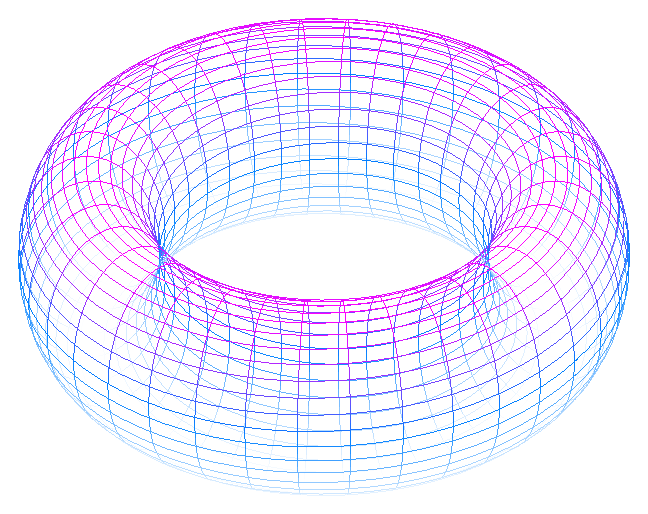
\includegraphics[scale=1]{torus.pdf}
\end{center}
\tableofcontents

\newpage
\section{Unit Circle}
The set $
\mathbb{S}^1 := \{ (x,y) \in \mathbb{R}^2 : x^2+y^2=1 \}$ is called the \textbf{unit circle}. 
\begin{center}
\begin{minipage}{.49\textwidth}\centering
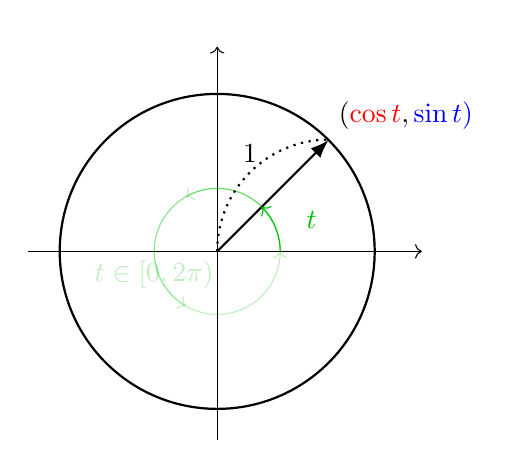
\begin{tikzpicture}[scale=2]
	% Unit circle
	\draw[thick] (0,0) circle(1);
	\draw[->] (-1.2,0) -- (1.3,0) node[right] {};
	\draw[->] (0,-1.2) -- (0,1.3) node[above] {};
	
	% Point at angle t
	\def\t{45}
	\draw[-Latex, thick] (0,0) -- ({cos(\t)}, {sin(\t)}) node[above right] {\(({\color{red}\cos t}, \color{blue}\sin t)\)};
	\draw[->, green!75!black, opacity=.25] (0.4,0) arc[start angle=0, end angle=120, radius=0.4] node[midway, below] {};
	\draw[->, green!75!black, opacity=.25] (0.4,0) arc[start angle=0, end angle=240, radius=0.4] node[midway, below] {};
	\draw[->, green!75!black, opacity=.25] (0.4,0) arc[start angle=0, end angle=360, radius=0.4] node[midway, below] {$t\in\intco{0,2\pi}$};
	\draw[->, green!75!black] (0.4,0) arc[start angle=0, end angle=\t, radius=0.4];
	\node[green!75!black] at (0.6,0.2) {\(t\)};
	% Curve labels
	%\node at (0,-1.5) {\textbf{Figure 1.} Trigonometric parametrization of the unit circle};
	
	\draw[-, dotted, thick] (0,0) arc[start angle=180, end angle=90, radius=.71] node[midway, above] {$1$};
\end{tikzpicture}
\end{minipage}\hfill
\begin{minipage}{.49\textwidth}\centering
	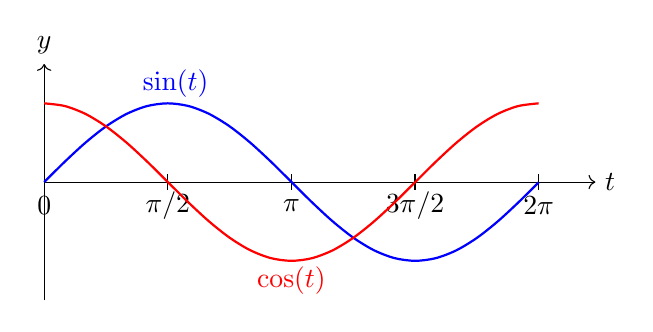
\begin{tikzpicture}[scale=1]
	% Draw axes
	\draw[->] (0,-1.5) -- (0,1.5) node[above] {\(y\)};
	\draw[->] (0,0) -- (7,0) node[right] {\(t\)};
	
	% Mark key points on the t-axis (0, pi/2, pi, 3pi/2, 2pi)
	\foreach \x in {0,1.57,3.14,4.71,6.28} {
		\draw (\x,0.1) -- (\x,-0.1);
	}
	\node at (0,-0.3) {\(0\)};
	\node at (1.57,-0.3) {\(\pi/2\)};
	\node at (3.14,-0.3) {\(\pi\)};
	\node at (4.71,-0.3) {\(3\pi/2\)};
	\node at (6.28,-0.3) {\(2\pi\)};
	
	% Draw sin(t) in blue
	\draw[domain=0:6.28, smooth, variable=\t, blue, thick] 
	plot ({\t},{sin(\t r)});
	\node[blue] at (1.67,1.25) {\(\sin(t)\)};
	
	% Draw cos(t) in red
	\draw[domain=0:6.28, smooth, variable=\t, red, thick] 
	plot ({\t},{cos(\t r)});
	\node[red] at (3.14,-1.25) {\(\cos(t)\)};
\end{tikzpicture}
\end{minipage}
\end{center}
The standard parametrization of \(\mathbb{S}^1\) is given by \[
t \mapsto (\cos t, \sin t), \quad t \in [0,2\pi),
\]
which implies the \emph{trigonometric identity} $\cos^2 t + \sin^2 t = 1$. The mapping \[
\fullfunction{\varphi}{\intco{0,2\pi}}{\mathbb{S}^1}{t}{(\cos t,\sin t)}.
\] provides a bijection between the half-open interval \(\intco{0,2\pi}\) and the unit circle $\mathbb{S}^1$.\par Geometrically, it represents the set of points at a fixed distance \(1\) from the origin in \(\mathbb{R}^2\), while algebraically it can be seen as a group under complex multiplication.
\begin{center}
	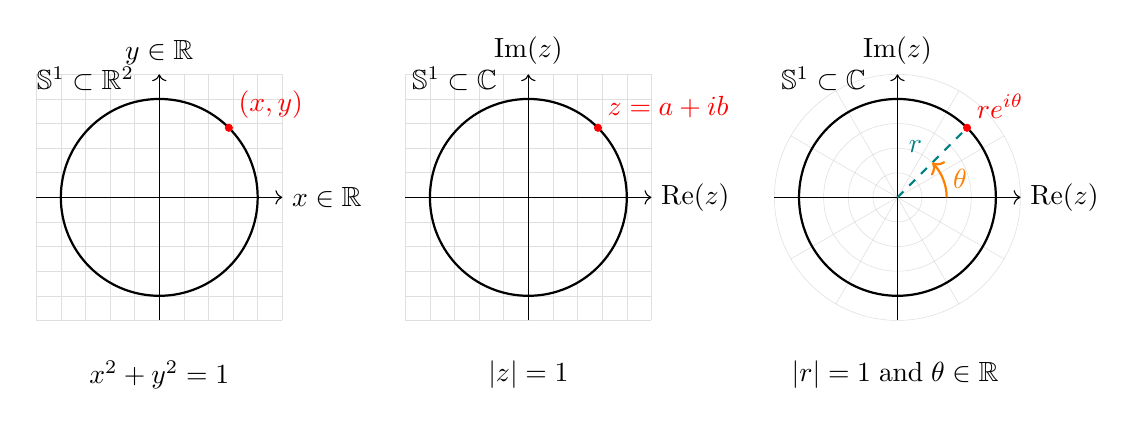
\begin{tikzpicture}[scale=1.25]
		% Left illustration: R^2 representation of the unit circle
		\begin{scope}[xshift=0cm]
			\draw[step=.25cm,gray!50,very thin,opacity=.5] (-1.25,-1.25) grid (1.25,1.25);
			% Axes for R^2
			\draw[->] (-1.25,0) -- (1.25,0) node[right] {$x\in\R$};
			\draw[->] (0,-1.25) -- (0,1.25) node[above] {$y\in\R$};
			% The unit circle in R^2
			\draw[thick] (0,0) circle (1cm);
			% Label the circle with its equation
			\node at (0,-1.8) {\(x^2 + y^2 = 1\)};
			\node at (-.75,1.2) {\(\mathbb{S}^1 \subset \mathbb{R}^2\)};
			\filldraw[red] (45:1cm) circle (1pt) node[above right] {\((x,y)\)};
		\end{scope}
		% Right illustration: Complex plane representation of the unit circle
		\begin{scope}[xshift=3.75cm]
			\draw[step=.25cm,gray!50,very thin,opacity=.5] (-1.25,-1.25) grid (1.25,1.25);
			% Axes for the complex plane
			\draw[->] (-1.25,0) -- (1.25,0) node[right] {\(\Re(z)\)};
			\draw[->] (0,-1.25) -- (0,1.25) node[above] {\(\Im(z)\)};
			% The unit circle in the complex plane
			\draw[thick] (0,0) circle (1cm);
			% Draw an arc to indicate the angle theta
			%		\draw[->, red] (0.5,0) arc (0:45:0.5);
			%		\node at (0.7,0.2) {\(\theta\)};
			% Mark and label a point on the circle corresponding to e^(i theta)
			\filldraw[red] (45:1cm) circle (1pt) node[above right] {\(z = a + ib\)};
			% Label the circle with its modulus condition
			\node at (0,-1.8) {\(|z| = 1\)};
			\node at (-.75,1.2) {\(\mathbb{S}^1 \subset \mathbb{C}\)};
			
			%		\filldraw[red] (1,1) circle (1.5pt) node[anchor=south west, black] {$$};
		\end{scope}
		\begin{scope}[xshift=7.5cm]
			% Draw concentric circles for radii 1 to 5
			\foreach \r in {.25,.5,...,1.25} {
				\draw[very thin, gray!50, opacity=.5] (0,0) circle (\r);
			}
			% Draw radial lines at every 30 degrees
			\foreach \angle in {0,30,...,360} {
				\draw[very thin, gray!50, opacity=.5] (0,0) -- (\angle:1.25);
			}
			
			% Axes for the complex plane
			\draw[->] (-1.25,0) -- (1.25,0) node[right] {\(\Re(z)\)};
			\draw[->] (0,-1.25) -- (0,1.25) node[above] {\(\Im(z)\)};
			% The unit circle in the complex plane
			\draw[thick] (0,0) circle (1cm);
			% Draw an arc to indicate the angle theta
			%		\draw[->, red] (0.5,0) arc (0:45:0.5);
			%		\node at (0.7,0.2) {\(\theta\)};
			% Mark and label a point on the circle corresponding to e^(i theta)
			\filldraw[red] (45:1cm) circle (1pt) node[above right] {\(re^{i\theta}\)};
			% Label the circle with its modulus condition
			\node at (0,-1.8) {\(\abs{r}=1\;\text{and}\;\theta \in \mathbb{R}\)};
			\node at (-.75,1.2) {\(\mathbb{S}^1 \subset \mathbb{C}\)};
			% draw radius
			\draw[dashed, thick, teal] (0,0) -- (.71,0.71) node[midway, above left] {$r$};
			% draw angle
			\draw[->, thick, orange] (0.5,0) arc (0:45:0.5) node[midway, right] {$\theta$};
		\end{scope}
	\end{tikzpicture}
\end{center}
The unit circle can be described in several equivalent ways. In \(\mathbb{R}^2\), it is given by:
\[
\mathbb{S}^1 = \{ (x,y) \in \mathbb{R}^2 : x^2 + y^2 = 1 \}.
\]
In the complex plane, we write:
\[
\mathbb{S}^1 = \{ z \in \mathbb{C} : |z| = 1 \} = \{ re^{i\theta} : \abs{r}=1\;\text{and}\;\theta \in \mathbb{R} \}.
\]
%These representations emphasize the geometric and algebraic property of \(S^1\).
We now show that \(\mathbb{S}^1\) forms a group under complex multiplication: \begin{enumerate}[(G1)]
	\item[(G0)] \textbf{(Closure)}\; Let $z_1 = e^{i\theta_1}$ and $z_2 = e^{i\theta_2} \in \mathbb{S}^1.$
	Then $z_1z_2 = e^{i\theta_1}e^{i\theta_2} = e^{i(\theta_1+\theta_2)}\in\mathbb{S}^1.$
	\item \textbf{(Associativity)}\; Let \(z_1=e^{i\theta_1}, z_2=e^{i\theta_2}, z_3=e^{i\theta_3} \in \mathbb{S}^1\) then \[
	(z_1z_2)z_3 = (e^{i\theta_1}e^{i\theta_2})e^{i\theta_3} = e^{i(\theta_1+\theta_2)}e^{i\theta_3} = e^{i(\theta_1+\theta_2+\theta_3)}=e^{i\theta_1}e^{i(\theta_2+\theta_3)}=e^{i\theta_1}(e^{i\theta_2}e^{i\theta_3})= z_1(z_2z_3).
	\]
	\item \textbf{(Identity Element)}\; For each \(z = e^{i\theta} \in \mathbb{S}^1\),
	\[
	1 \cdot z = e^{i0}e^{i\theta} = e^{i(0+\theta)}=e^{i\theta} = z,
	\]
	and similarly \(z \cdot 1 = z\).
	\item \textbf{(Inverses)}\; For any \(z = e^{i\theta} \in \mathbb{S}^1\), its inverse is given by $
	z^{-1} = e^{-i\theta},$ since
	\[
	z \cdot z^{-1} = e^{i\theta}e^{-i\theta} = e^{i(\theta-\theta)} = e^{i\cdot 0} = 1.
	\]
	Notice that \(e^{-i\theta} \in \mathbb{S}^1\) as well.
\end{enumerate}
We show that \textbf{multiplication on the circle group is equivalent to addition of angles}:
let \begin{align*}
	z_1&= r_1e^{i\theta_1}=r_1\of{\cos\theta_1+i\sin\theta_1}\in\C\;\text{and}\\
	z_2&= r_2e^{i\theta_2}=r_2\of{\cos\theta_2+i\sin\theta_2}\in\C.
\end{align*} Then \begin{align*}
	z_1\cdot z_2=r_1e^{i\theta_1}\cdot r_2e^{i\theta_2}=&=r_1r_2\of{\cos\theta_1+i\sin\theta_1}\of{\cos\theta_2+i\sin\theta_2}\\
	&=r_1r_2\left[\of{\cos\theta_1\cos\theta_2-\sin\theta_1\sin\theta_2}+i\of{\cos\theta_1\sin\theta_2+\sin\theta_1\cos\theta_2}\right]\\
	&=r_1r_2\left[\cos\of{\theta_1+\theta_2}+i\sin\of{\theta_1+\theta_2}\right]\\
	&=r\of{\cos\theta+\sin\theta}\ \text{with}\ \begin{cases}
		r=r_1r_2\\
		\theta=\theta_1+\theta_2.
	\end{cases}
\end{align*}
\begin{center}
	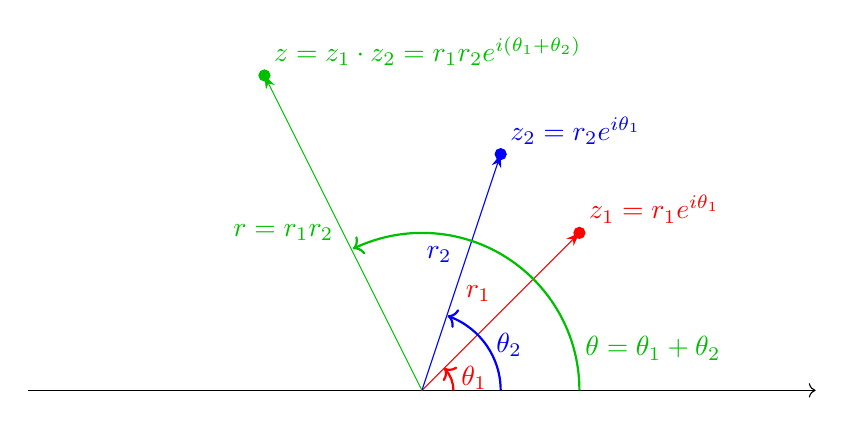
\begin{tikzpicture}[scale=2]
		\draw[->] (-2.5,0) -- (2.5,0) node[right] {};
		\filldraw[red] (1,1) circle (1pt) node[anchor=south west] {$z_1=r_1e^{i\theta_1}$};
		\filldraw[blue] (.5,1.5) circle (1pt) node[anchor=south west] {$z_2=r_2e^{i\theta_1}$};
		\filldraw[green!75!black] (-1,2) circle (1pt) node[anchor=south west] {$z=z_1\cdot z_2=r_1r_2e^{i(\theta_1+\theta_2)}$};
		
		\draw[-Stealth, red] (0,0) -- (1,1) node[midway, above left] {$r_1$};
		\draw[-Stealth, blue] (0,0) -- (.5,1.5) node[midway, above left] {$r_2$};
		\draw[-Stealth, green!75!black] (0,0) -- (-1,2) node[midway, left] {$r=r_1r_2$};
		\draw[->, thick, red] (.2,0) arc (0:45:.2) node[midway, right] {$\theta_1$};
		\draw[->, thick, blue] (.5,0) arc (0:71:.5) node[midway, right] {$\theta_2$};
		\draw[->, thick, green!75!black] (1,0) arc (0:116:1) node[midway, below right=1.25cm] {$\theta=\theta_1+\theta_2$};
	\end{tikzpicture}
\end{center}

\newpage
\subsection{Quotient Space}
\begin{center}
\begin{tikzpicture}[scale=1]
	\draw[-, thick, blue] (-2,0) -- (2,0);
	\filldraw[fill=white, draw=red] (-2,0) circle (2pt) node[above, red] {$0$};
%	\fill[teal] (-.67,0) circle (2pt) node[above] {$1/3$};
%	\fill[orange] (.67,0) circle (2pt) node[above] {$2/3$};
	\filldraw[fill=white, draw=red] (2,0) circle (2pt) node[above, red] {$1$};
\begin{scope}[xshift=6cm]
%	\draw[step=.5cm,gray!50,very thin,opacity=.5] (-3,-3) grid (3,3);
	
%	\draw[->] (-3,0) -- (3,0) node[right] {};
%	\draw[->] (0,-3) -- (0,3) node[above] {};
	
	\draw[-Stealth, thick] (0,2) arc (90:450:2);
	\draw[-Stealth, thick] (0,2) arc (90:-270:2);
	\filldraw[red] (0,2) circle (2pt);
	\node[above, red] at (0,2) {\(\,[0]=[1]\)};
\end{scope}
\begin{scope}[xshift=12cm]
	\draw[-, thick, blue] (0,2) arc (90:450:2) node[above] {$\mathbb{S}^1$};
\end{scope}
\end{tikzpicture}
\end{center}
\begin{center}
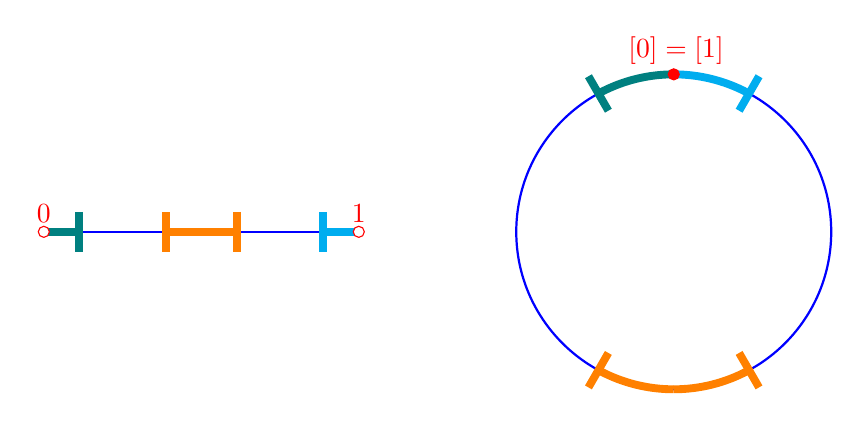
\begin{tikzpicture}[scale=1]
\draw[-, thick, blue] (-2,0) -- (2,0);
\draw[-|, line width=1mm, teal] (-2,0) -- (-1.5,0);
\draw[-|, line width=1mm, cyan] (2,0) -- (1.5,0);
\draw[|-|, line width=1mm, orange] (-.5,0) -- (.5,0);
\filldraw[fill=white, draw=red] (-2,0) circle (2pt) node[above, red] {$0$};
\filldraw[fill=white, draw=red] (2,0) circle (2pt) node[above, red] {$1$};
\begin{scope}[xshift=6cm]
	\draw[-, thick, blue] (0,2) arc (90:450:2);
	\draw[-|, line width=1mm, teal] (0,2) arc (90:120:2);
	\draw[-|, line width=1mm, cyan] (0,2) arc (90:60:2);
	\draw[-|, line width=1mm, orange] (0,-2) arc (270:300:2);
	\draw[-|, line width=1mm, orange] (0,-2) arc (270:240:2);
	
	\filldraw[red] (0,2) circle (2pt);
	\node[above, red] at (0,2) {\(\,[0]=[1]\)};
\end{scope}
\end{tikzpicture}
\end{center}
Let \[
\pi: \mathbb{R} \to \mathbb{R}/\mathbb{Z},\quad x \mapsto x+\mathbb{Z},
\] be the canonical projection onto the quotient group, where the equivalence relation is given by
\[
x \sim y \quad \Longleftrightarrow \quad x-y \in \mathbb{Z}.
\]
Denote by
\[
[x] = \{\, y \in \mathbb{R} \mid y \sim x \,\} = x + \mathbb{Z}
\]
the equivalence class of \(x\). Then $\mathbb{R}/\mathbb{Z} = \{ [x] : x \in \mathbb{R} \}.$
Thus, each element of \(\mathbb{R}/\mathbb{Z}\) is a coset of the subgroup \(\mathbb{Z}\) in \(\mathbb{R}\).
Consider the canonical projection map
\[
\pi: \mathbb{R} \to \mathbb{R}/\mathbb{Z}, \quad \pi(x) = [x].
\]
The topology on \(\mathbb{R}/\mathbb{Z}\) is defined as the **quotient topology** induced by \(\pi\). That is, a subset \(U \subseteq \mathbb{R}/\mathbb{Z}\) is declared open if and only if its preimage under \(\pi\) is open in \(\mathbb{R}\); symbolically,
\[
U \in \tau \quad \Longleftrightarrow \quad \pi^{-1}(U) \in \tau_{\mathbb{R}},
\]
where \(\tau_{\mathbb{R}}\) is the standard topology on \(\mathbb{R}\) (i.e., the topology generated by the open intervals).

3. Formal Definition Summary

- **Set:**  
\[
\mathbb{R}/\mathbb{Z} = \{\, [x] : x \in \mathbb{R} \,\},
\]
where \([x] = \{ x + n : n \in \mathbb{Z} \}\).

- **Topology:**  
The topology \(\tau\) on \(\mathbb{R}/\mathbb{Z}\) is given by
\[
\tau = \{\, U \subseteq \mathbb{R}/\mathbb{Z} \mid \pi^{-1}(U) \in \tau_{\mathbb{R}} \,\}.
\]
This makes \(\pi\) a continuous, surjective map, and by definition, \(\mathbb{R}/\mathbb{Z}\) becomes a topological space known as the quotient space of \(\mathbb{R}\) by \(\mathbb{Z}\).

4. Additional Comments

It is a classical result that \(\mathbb{R}/\mathbb{Z}\) is homeomorphic to the circle \(S^1\). One explicit homeomorphism is given by
\[
\varphi: \mathbb{R}/\mathbb{Z} \to S^1, \quad \varphi([x]) = e^{2\pi i x},
\]
which is continuous, bijective, and has a continuous inverse.

This completes the formal construction of the topological space \(\mathbb{R}/\mathbb{Z}\) by specifying both its underlying set and the quotient topology derived from the standard topology on \(\mathbb{R}\).

It is well known that the topological space \(\mathbb{R}/\mathbb{Z}\) is homeomorphic to the circle \(S^1\). For instance, define
\[
\varphi: \mathbb{R}/\mathbb{Z} \to S^1,\quad \varphi(x+\mathbb{Z}) = e^{2\pi i x}.
\]
Then \(\varphi\) is a continuous bijection with continuous inverse, hence a homeomorphism.

\ \\
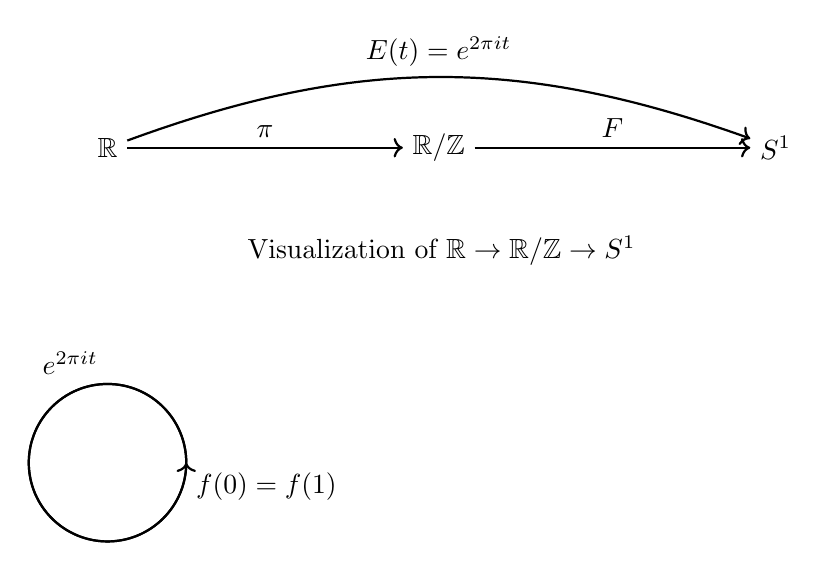
\begin{tikzpicture}[node distance=3.5cm, auto]
	% Main Diagram: Relationship between R, R/Z, and S^1
	\node (R) {$\mathbb{R}$};
	\node (RZ) [right=of R] {$\mathbb{R}/\mathbb{Z}$};
	\node (S1) [right=of RZ] {$S^1$};
	
	% Arrows representing the maps
	\draw[->, thick] (R) -- node[above] {$\pi$} (RZ);
	\draw[->, thick, bend left=20] (R) to node[above] {$E(t)=e^{2\pi it}$} (S1);
	\draw[->, thick] (RZ) -- node[above] {$F$} (S1);
	
	% Inset Diagram: Visualization of the Exponential Map on S^1
	\begin{scope}[shift={(0,-4)}]
		% Draw unit circle
		\draw[thick] (0,0) circle (1);
		% Draw an arrow along the circle to illustrate the wrapping
		\draw[->, thick] (1,0) arc (0:360:1);
		% Mark the identified point f(0)=f(1)
		\node at (1,0) [below right] {$f(0)=f(1)$};
		% Label an arbitrary point on the circle
		\node at (0,1) [above left] {$e^{2\pi it}$};
	\end{scope}
	
	% Optional descriptive label for the whole diagram
	\node at ($(R)!0.5!(S1)$) [below=1cm] {Visualization of $\mathbb{R} \to \mathbb{R}/\mathbb{Z} \to S^1$};
\end{tikzpicture}

\newpage
\subsection{Linear Approximation}
\begin{center}
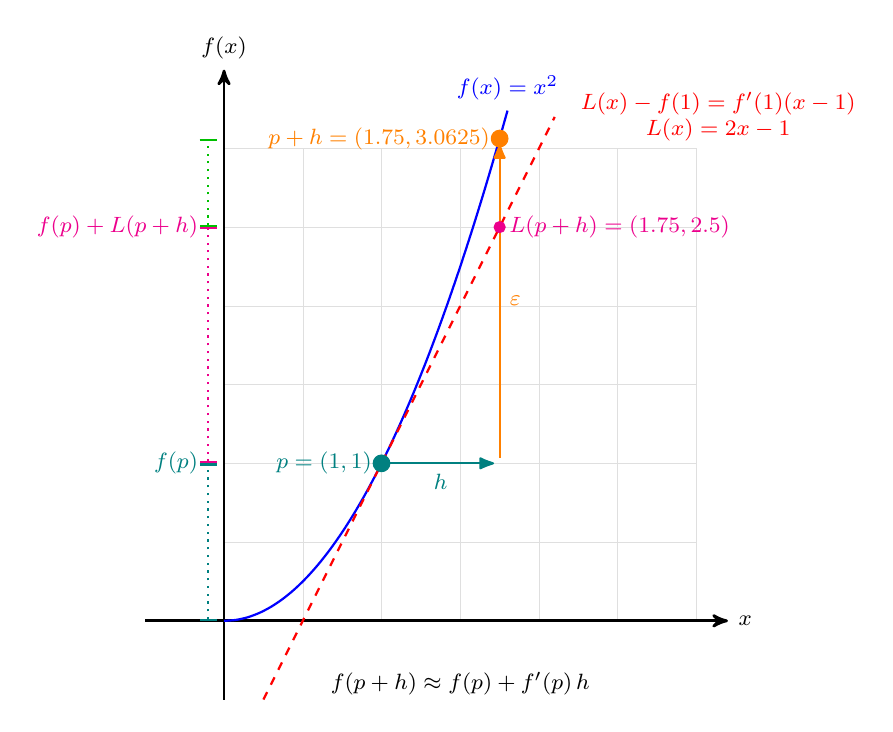
\begin{tikzpicture}[scale=2, 
	every node/.style={font=\footnotesize},
	axis/.style={->, >=stealth', line width=1pt},
	function/.style={domain=0:1.8, smooth, variable=\x, blue, thick},
	tangent/.style={red, thick, dashed},
	error/.style={orange, thick, -{Latex[round]}},
	point/.style={fill=black, circle, inner sep=1.5pt}]
	
	\draw[step=.5cm,gray!50,very thin,opacity=.5] (0,0) grid (3,3);
	
	% Draw coordinate axes
	\draw[axis] (-0.5,0) -- (3.2,0) node[right] {$x$};
	\draw[axis] (0,-0.5) -- (0,3.5) node[above] {$f(x)$};
	
	% Plot the function f(x) = x^2
	\draw[function] plot (\x, {\x*\x}) node[above] {$f(x)=x^2$};
	
	% Draw the tangent line at p.
	% f'(x) = 2x, so at p, f'(1)=2 and the tangent line is L(x)= 1+2(x-1)=2x-1.
	\draw[tangent,domain=.25:2.1] plot (\x, {2*\x - 1}) node[right, xshift=2mm, align=center] {$L(x)-f(1)=f'(1)(x-1)$\\$L(x)=2x-1$};
	
	\coordinate (p) at (1,1);
	\coordinate (q) at (1.75, {1.75*1.75});
	\coordinate (r) at (1.75,1);
	\draw[error, shorten <=2pt, shorten >=2pt, teal] (p) -- node[below] {$h$} (r);
	\draw[error, shorten <=2pt, shorten >=2pt, orange] (r) -- node[right] {$\varepsilon$} (q);
	
	% Mark the corresponding point on the tangent line at x=1.5, which is L(1.5) = (1.5,2).
	\coordinate (s) at (1.75, {2*1.75 - 1});
	\draw[point, magenta] (s) circle (1pt);
	\node[right, magenta] at (s) {$L(p+h)=(1.75,2.5)$};
	
%	%Optionally, illustrate the curvilinear path along the graph from p to q.
%	\draw[very thin, dashed] (p) .. controls (1.2, 1.2) and (1.3, 1.7) .. (q);
	
	% Annotation of the linear approximation formula
	\node at (1.5, -0.4) {$f(p+h) \approx f(p) + f'(p)\,h$};

	\draw[point, teal] (p) circle (1.5pt);
	\node[left, teal] at (p) {$p=(1,1)$};
	\draw[point, orange] (q) circle (1.5pt);
	\node[left, orange] at (q) {$p+h=(1.75,3.0625)$};
	\draw[teal, dotted, thick, |-|] (-.1, 0) -- (-.1, 1) node[left] {$f(p)$};
	\draw[magenta, dotted, thick, |-|] (-.1, 1) -- (-.1, 2.5) node[left] {$f(p)+L(p+h)$};
	\draw[green!75!black, dotted, thick, |-|] (-.1, 2.5) -- (-.1, 3.0625);
\end{tikzpicture}
\end{center}

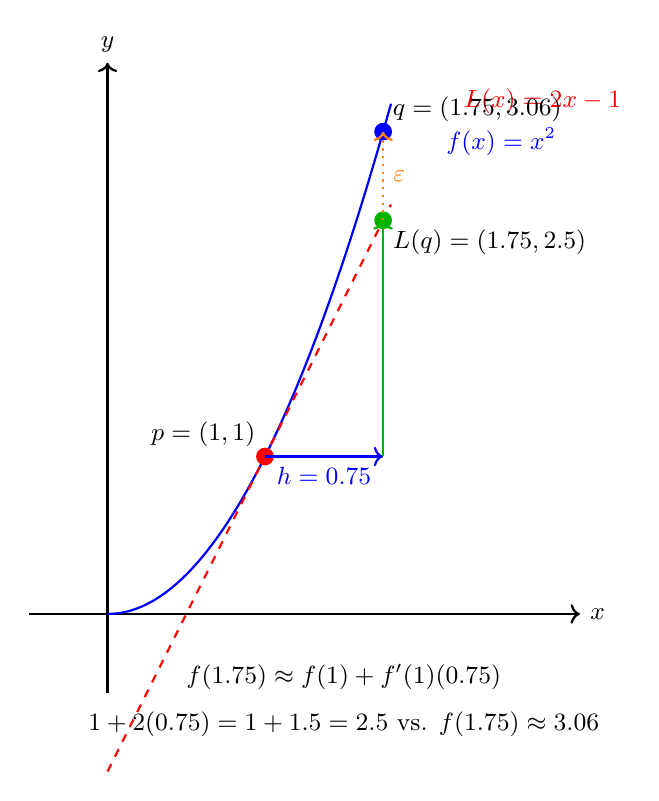
\begin{tikzpicture}[scale=2, every node/.style={font=\small}]
	
	% Draw coordinate axes
	\draw[->, thick] (-0.5,0) -- (3,0) node[right] {$x$};
	\draw[->, thick] (0,-0.5) -- (0,3.5) node[above] {$y$};
	
	% Plot the function f(x)=x^2 in blue
	\draw[domain=0:1.8, smooth, variable=\x, blue, thick] plot (\x, {\x*\x});
	\node[blue] at (2.5, 6.0/2) {$f(x)=x^2$};
	
	% Define the point p = (1, f(1)) = (1,1)
	\coordinate (p) at (1,1);
	\filldraw[red] (p) circle (1.5pt);
	\node[above left] at (p) {$p=(1,1)$};
	
	% Draw the tangent line at p.
	% f'(1)=2, so tangent line L(x)= 1 + 2(x-1)=2x-1.
	\draw[red, dashed, thick, domain=0:1.8] plot (\x, {2*\x - 1});
	\node[red] at (2.2, {2*2.2 - 1}) [below right] {$L(x)=2x-1$};
	
	% Displacement: h = 0.75, so new x-coordinate is 1.75.
	% Actual point on the curve: q = (1.75, f(1.75))
	\coordinate (q) at (1.75, {1.75*1.75});
	\filldraw[blue] (q) circle (1.5pt);
	\node[above right] at (q) {$q=(1.75,3.06)$};
	
	% Compute tangent line value at x=1.75: L(1.75)=2*1.75-1=2.5.
	\coordinate (r) at (1.75, {2*1.75 - 1});
	\filldraw[green!70!black] (r) circle (1.5pt);
	\node[below right] at (r) {$L(q)=(1.75,2.5)$};
	
	% Draw horizontal arrow representing h from p to a vertical line at x=1.75.
	\draw[->, thick, blue] (p) -- (1.75,1) node[midway, below] {$h=0.75$};
	
	% Draw vertical arrow from (1.75,1) up to the tangent line point r.
	\draw[->, thick, green!70!black] (1.75,1) -- (r);
	
	% Draw vertical dotted arrow from tangent line point r to the actual curve point q.
	\draw[dotted, thick, ->, orange] (r) -- (q) node[midway, right] {$\varepsilon$};
	
	% Annotate the linear approximation formula.
	\node at (1.5,-0.4) {$f(1.75)\approx f(1)+f'(1)(0.75)$};
	\node at (1.5,-0.7) {$1+2(0.75)=1+1.5=2.5$ vs. $f(1.75)\approx3.06$};
	
\end{tikzpicture}

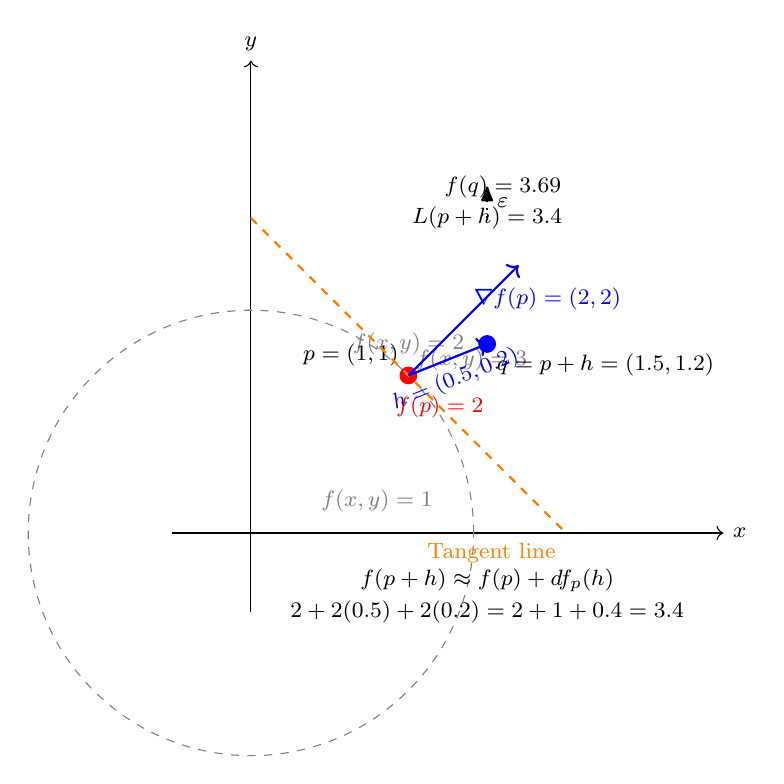
\begin{tikzpicture}[scale=2, every node/.style={font=\footnotesize}]
	
	% Draw coordinate axes
	\draw[->] (-0.5,0) -- (3,0) node[right] {$x$};
	\draw[->] (0,-0.5) -- (0,3) node[above] {$y$};
	
	% Draw level curves of f(x,y)=x^2+y^2.
	% Level curves: x^2+y^2 = c for various values of c.
	\foreach \c in {2} {
		\draw[gray, dashed] (0,0) circle ({sqrt(\c)});
	}
	% Label a couple of level curves
	\node[gray] at (0.8,0.2) {$f(x,y)=1$};
	\node[gray] at (1,1.2) {$f(x,y)=2$};
	\node[gray] at (1.4,1.1) {$f(x,y)=3$};
	
	% Mark the point p=(1,1) and label f(p)=2.
	\coordinate (p) at (1,1);
	\filldraw[red] (p) circle (1.5pt);
	\node[above left] at (p) {$p=(1,1)$};
	\node[red] at (1.2,0.8) {$f(p)=2$};
	
	% Draw the gradient vector at p: grad f = (2x,2y) = (2,2) at p.
	\draw[->, blue, thick] (p) -- ($(p)+(0.7,0.7)$) node[midway, above right] {$\nabla f(p)=(2,2)$};
	
	% Draw the tangent line to the level curve at p.
	% The tangent line is perpendicular to the gradient. One perpendicular direction to (2,2) is (-1,1).
	\draw[orange, thick, dashed] ($(p)+(-1,1)$) -- ($(p)+(1,-1)$) node[below left] {Tangent line};
	
	% Choose a displacement h=(0.5,0.2) so that q=p+h=(1.5,1.2).
	\coordinate (q) at (1.5,1.2);
	\filldraw[blue] (q) circle (1.5pt);
	\node[below right] at (q) {$q=p+h=(1.5,1.2)$};
	
	% Draw arrow for displacement h from p to q.
	\draw[->, thick, blue] (p) -- (q) node[midway, below, sloped] {$h=(0.5,0.2)$};
	
	% Calculate f(q)=1.5^2+1.2^2 = 2.25+1.44=3.69 and annotate.
	\node at (1.6,2.2) {$f(q)=3.69$};
	
	% Linear approximation: the differential df_p = (2,2). For h=(0.5,0.2),
	% df_p(h)=2*0.5+2*0.2=1.0+0.4=1.4, so the tangent plane predicts
	% f(p+h) ≈ f(p)+df_p(h)=2+1.4=3.4.
	\node at (1.5, 2.0) {$L(p+h)=3.4$};
	
	% Draw a dotted arrow to indicate the vertical error between the true value and the linear prediction.
	\draw[dotted, thick, -{Latex[round]}] (1.5,2.0) -- (1.5,2.2) node[midway, right] {$\varepsilon$};
	
	% Annotate the linear approximation formula
	\node at (1.5,-0.3) {$f(p+h) \approx f(p)+df_p(h)$};
	\node at (1.5,-0.5) {$2+2(0.5)+2(0.2)=2+1+0.4=3.4$};
	
\end{tikzpicture}

Below is a detailed explanation, along with a concrete calculation, that defines what a differential is in the context of smooth manifolds.

 1. Differential as the Best Linear Approximation

Let \( f \colon M \to \mathbb{R} \) be a smooth function defined on a smooth manifold \(M\). The **differential of \( f \) at a point \( p \in M \)**, denoted by \( df_p \), is defined as the best linear approximation to \( f \) near \( p \). Concretely, \( df_p \) is a linear map
\[
df_p \colon T_pM \to \mathbb{R},
\]
where \( T_pM \) is the tangent space at \( p \).

 1.1. Definition via Curves

One way to define \( df_p \) is by using smooth curves. Let \( v \in T_pM \) be a tangent vector, and let \(\gamma \colon (-\varepsilon,\varepsilon) \to M\) be any smooth curve with
\[
\gamma(0) = p \quad \text{and} \quad \gamma'(0) = v.
\]
Then, the differential \( df_p \) applied to \( v \) is given by:
\[
df_p(v) = \left. \frac{d}{dt} \right|_{t=0} f\bigl(\gamma(t)\bigr).
\]
This derivative is independent of the particular choice of curve \(\gamma\) as long as it has the correct initial velocity \( v \).

 1.2. Linear Approximation

In elementary calculus for functions \( f \colon \mathbb{R} \to \mathbb{R} \), the derivative \( f'(x) \) gives the linear (first-order) approximation:
\[
f(x+h) \approx f(x) + f'(x)h \quad \text{for small } h.
\]
In higher dimensions, \( df_p \) generalizes this idea. It is the linear map that approximates the change in \( f \) near \( p \). If \( p \in \mathbb{R}^n \) and \( v \in \mathbb{R}^n \), then
\[
f(p+v) \approx f(p) + df_p(v).
\]

2. Differential in Local Coordinates

If \( (U, \varphi) \) is a coordinate chart around \( p \) with coordinates \( (x^1,\dots,x^n) \), then \( f \) can be written locally as a function \( f(x^1,\dots,x^n) \). In these coordinates, the differential is given by:
\[
df = \frac{\partial f}{\partial x^1} dx^1 + \frac{\partial f}{\partial x^2} dx^2 + \cdots + \frac{\partial f}{\partial x^n} dx^n.
\]
Here, \( dx^1, dx^2, \dots, dx^n \) are the canonical 1–forms associated with the coordinate functions. For a tangent vector \( v = (v^1,\dots,v^n) \) (which in these coordinates is written as \( v = v^i \partial/\partial x^i \)), we have:
\[
df_p(v) = \sum_{i=1}^n \frac{\partial f}{\partial x^i}(p)\, v^i.
\]

 3. Differential as a Section of the Cotangent Bundle

The assignment \( p \mapsto df_p \) defines a smooth section of the cotangent bundle \( T^*M \). This means that \( df \) is a 1–form on \( M \). In other words, it assigns to each point \( p \) a covector (a linear functional on \( T_pM \)) in a smooth (i.e. differentiable) manner.

4. Concrete Calculation Example

Consider the function \( f \colon \mathbb{R}^2 \to \mathbb{R} \) given by
\[
f(x,y) = x^2 + y^2.
\]
Let \( p = (1,2) \). We want to compute \( df_p \).

1. **Compute the Partial Derivatives:**

\[
\frac{\partial f}{\partial x}(x,y) = 2x,\quad \frac{\partial f}{\partial y}(x,y) = 2y.
\]

2. **Evaluate at \( p = (1,2) \):**

\[
\frac{\partial f}{\partial x}(1,2) = 2, \quad \frac{\partial f}{\partial y}(1,2) = 4.
\]

3. **Express \( df \) in Coordinates:**

\[
df = 2x\,dx + 2y\,dy.
\]
At \( p \), this becomes:
\[
df_{(1,2)} = 2\,dx + 4\,dy.
\]

4. **Apply \( df_p \) to a Tangent Vector:**

Let \( v = (3, -1) \in T_{(1,2)}\mathbb{R}^2 \). Then:
\[
df_{(1,2)}(v) = 2\cdot 3 + 4\cdot (-1) = 6 - 4 = 2.
\]

This number \( 2 \) is the rate at which \( f \) increases in the direction of the vector \( v \) at the point \( (1,2) \).

 Summary

- **Differential \( df_p \):**  
For a smooth function \( f \colon M \to \mathbb{R} \), the differential at \( p \), \( df_p \), is a linear map from the tangent space \( T_pM \) to \( \mathbb{R} \) that gives the best linear approximation of \( f \) near \( p \).

- **Definition via Curves:**  
It is defined by
\[
df_p(v) = \left. \frac{d}{dt} \right|_{t=0} f(\gamma(t)),
\]
for any curve \( \gamma \) with \( \gamma(0)=p \) and \( \gamma'(0)=v \).

- **Local Expression:**  
In local coordinates,
\[
df = \sum_{i=1}^n \frac{\partial f}{\partial x^i}\,dx^i,
\]
which acts on tangent vectors by the dot product with the gradient of \( f \).

- **Global Perspective:**  
The map \( p \mapsto df_p \) defines a smooth section of the cotangent bundle \( T^*M \), and thus \( df \) is a 1–form on \( M \).

This detailed explanation, along with the concrete calculation for a function on \(\mathbb{R}^2\), illustrates what a differential is and why it is such a central concept in differential geometry and analysis.


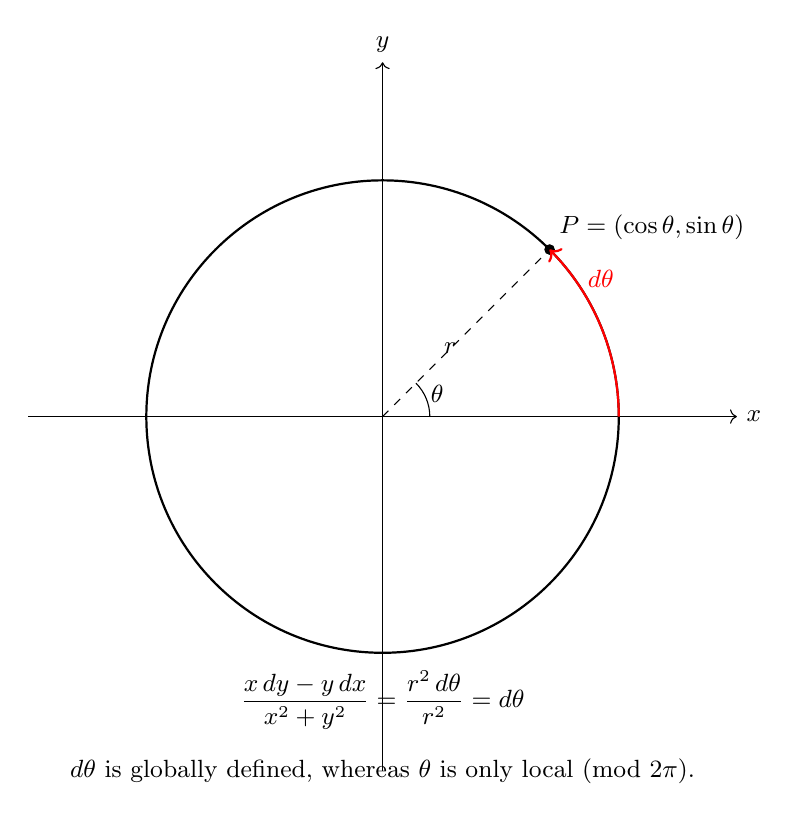
\begin{tikzpicture}[scale=3, every node/.style={font=\small}]
	
	% Draw coordinate axes.
	\draw[->] (-1.5,0) -- (1.5,0) node[right] {$x$};
	\draw[->] (0,-1.5) -- (0,1.5) node[above] {$y$};
	
	% Draw the unit circle: x^2+y^2=1.
	\draw[thick] (0,0) circle (1);
	
	% Define an angle t in degrees.
	\def\angle{45}
	
	% Compute the point P on the circle corresponding to the angle t.
	\coordinate (P) at ({cos(\angle)}, {sin(\angle)});
	
	% Draw the radial line from the origin to point P.
	\draw[dashed] (0,0) -- (P) node[midway, below left] {$r$};
	
	% Mark and label the point P.
	\filldraw (P) circle (0.02) node[above right] {$P=(\cos\theta,\sin\theta)$};
	
	% Draw a small arc at the origin to indicate the angle theta.
	\draw (0.2,0) arc (0:\angle:0.2);
	\node at ({0.25*cos(\angle/2)},{0.25*sin(\angle/2)}) {$\theta$};
	
	% Illustrate the arc element along the unit circle.
	\draw[red, thick, ->] (1,0) arc (0:\angle:1);
	\node[red] at ({cos(\angle/2)},{sin(\angle/2)+0.2}) {$d\theta$};
	
	% Annotation showing the calculation in polar coordinates.
	\node[align=center] at (0,-1.2) 
	{\small $\displaystyle \frac{x\,dy-y\,dx}{x^2+y^2}=\frac{r^2\,d\theta}{r^2}=d\theta$};
	
	% Additional note: dtheta is well-defined.
	\node[align=center] at (0,-1.5) 
	{\small $d\theta$ is globally defined, whereas $\theta$ is only local (mod $2\pi$).};
	
\end{tikzpicture}


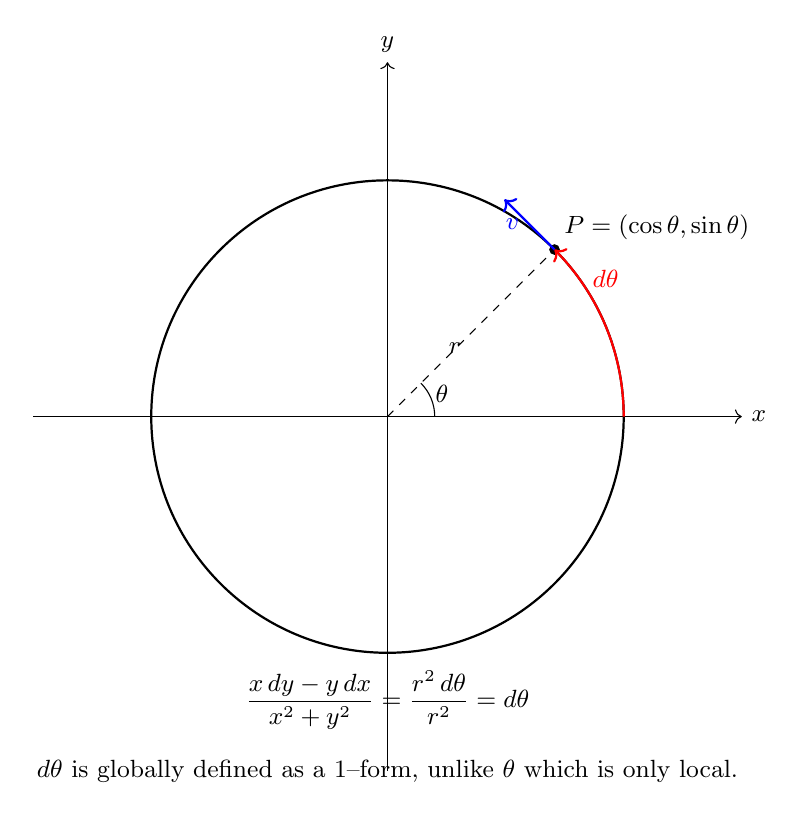
\begin{tikzpicture}[scale=3, every node/.style={font=\small}]
	
	% Draw coordinate axes.
	\draw[->] (-1.5,0) -- (1.5,0) node[right] {$x$};
	\draw[->] (0,-1.5) -- (0,1.5) node[above] {$y$};
	
	% Draw the unit circle: x^2+y^2=1.
	\draw[thick] (0,0) circle (1);
	
	% Define an angle theta in degrees.
	\def\angle{45}
	
	% Compute the point P on the circle corresponding to the angle theta.
	\coordinate (P) at ({cos(\angle)}, {sin(\angle)});
	
	% Draw the radial line from the origin to point P.
	\draw[dashed] (0,0) -- (P) node[midway, below left] {$r$};
	
	% Mark and label the point P.
	\filldraw (P) circle (0.02) node[above right] {$P=(\cos\theta,\sin\theta)$};
	
	% Draw the tangent vector at P.
	% For a point at angle theta, a unit tangent vector is given by (-sin theta, cos theta).
	\draw[->, blue, thick] (P) -- ++({-sin(\angle)*0.3}, {cos(\angle)*0.3})
	node[midway, left] {$v$};
	
	% Draw a small arc at the origin to indicate the angle theta.
	\draw (0.2,0) arc (0:\angle:0.2);
	\node at ({0.25*cos(\angle/2)},{0.25*sin(\angle/2)}) {$\theta$};
	
	% Illustrate the arc element along the unit circle.
	\draw[red, thick, ->] (1,0) arc (0:\angle:1);
	\node[red] at ({cos(\angle/2)},{sin(\angle/2)+0.2}) {$d\theta$};
	
	% Annotation: Show the algebraic conversion in polar coordinates.
	\node[align=center] at (0,-1.2) 
	{\small $\displaystyle \frac{x\,dy-y\,dx}{x^2+y^2}=\frac{r^2\,d\theta}{r^2}=d\theta$};
	
	% Additional note: why dθ and not θ.
	\node[align=center] at (0,-1.5) 
	{\small $d\theta$ is globally defined as a 1–form, unlike $\theta$ which is only local.};
	
\end{tikzpicture}

On \(\mathbb{R}^2 \setminus \{0\}\), when we express the coordinates in polar form with
\[
x = r\cos\theta,\quad y = r\sin\theta,
\]
the 1–form
\[
\omega = \frac{x\,dy - y\,dx}{x^2+y^2}
\]
simplifies to
\[
d\theta.
\]

 Verification in Polar Coordinates

1. **Express \(dx\) and \(dy\) in polar coordinates:**
\[
dx = \cos\theta\,dr - r\sin\theta\,d\theta,\quad dy = \sin\theta\,dr + r\cos\theta\,d\theta.
\]

2. **Compute the numerator:**
\[
\begin{aligned}
	x\,dy - y\,dx &= r\cos\theta \,(\sin\theta\,dr + r\cos\theta\,d\theta) - r\sin\theta\,(\cos\theta\,dr - r\sin\theta\,d\theta) \\
	&= r\cos\theta\sin\theta\,dr + r^2\cos^2\theta\,d\theta - r\sin\theta\cos\theta\,dr + r^2\sin^2\theta\,d\theta \\
	&= r^2 (\cos^2\theta + \sin^2\theta)\,d\theta \\
	&= r^2\,d\theta.
\end{aligned}
\]

3. **Compute the denominator:**
\[
x^2+y^2 = r^2\cos^2\theta + r^2\sin^2\theta = r^2.
\]

4. **Combine the results:**
\[
\omega = \frac{r^2\,d\theta}{r^2} = d\theta.
\]

 Interpretation

- **\(d\theta\):**  
This differential represents the infinitesimal change in the angular coordinate \(\theta\). Although the function \(\theta\) is not globally well-defined on \(\mathbb{R}^2 \setminus \{0\}\) (because angles are defined modulo \(2\pi\)), its differential \(d\theta\) is a well-defined 1–form on this space.

- **Winding Number:**  
When you integrate \(\omega\) (or equivalently \(d\theta\)) over a closed curve \(\gamma\) in \(\mathbb{R}^2 \setminus \{0\}\),
\[
\int_\gamma \omega = \int_\gamma d\theta,
\]
you obtain the total angular change along \(\gamma\). Normalizing this by \(2\pi\) gives the winding number of \(\gamma\) about the origin.

In summary, on \(\mathbb{R}^2 \setminus \{0\}\), the form
\[
\frac{x\,dy - y\,dx}{x^2+y^2}
\]
is equivalent to \(d\theta\) in polar coordinates.


\begin{tikzpicture}[scale=3, every node/.style={font=\small}]
	
	% Draw coordinate axes.
	\draw[->] (-1.5,0) -- (1.5,0) node[right] {$x$};
	\draw[->] (0,-1.5) -- (0,1.5) node[above] {$y$};
	
	% Draw the unit circle: x^2+y^2=1.
	\draw[thick] (0,0) circle (1);
	
	% Define an angle theta in degrees.
	\def\angle{45}
	
	% Compute the point P on the circle corresponding to the angle theta.
	\coordinate (P) at ({cos(\angle)}, {sin(\angle)});
	
	% Draw the radial line from the origin to point P.
	\draw[dashed] (0,0) -- (P) node[midway, below left] {$r$};
	
	% Mark and label the point P.
	\filldraw (P) circle (0.02) node[above right] {$P=(\cos\theta,\sin\theta)$};
	
	% Draw the tangent vector at P.
	% For a point at angle theta, a unit tangent vector is given by (-sin theta, cos theta).
	\draw[->, blue, thick] (P) -- ++({-sin(\angle)*0.3}, {cos(\angle)*0.3})
	node[midway, left] {$v$};
	
	% Draw a small arc at the origin to indicate the angle theta.
	\draw (0.2,0) arc (0:\angle:0.2);
	\node at ({0.25*cos(\angle/2)},{0.25*sin(\angle/2)}) {$\theta$};
	
	% Illustrate the arc element along the unit circle.
	\draw[red, thick, ->] (1,0) arc (0:\angle:1);
	\node[red] at ({cos(\angle/2)},{sin(\angle/2)+0.2}) {$d\theta$};
	
	% Annotation: Show the algebraic conversion in polar coordinates.
	\node[align=center] at (0,-1.2) 
	{\small $\displaystyle \frac{x\,dy-y\,dx}{x^2+y^2}=\frac{r^2\,d\theta}{r^2}=d\theta$};
	
\end{tikzpicture}


The 1–form 
\[
\omega = \frac{x\,dy - y\,dx}{x^2+y^2}
\]
can seem mysterious at first, but it becomes clear when we change to polar coordinates. Here is a step-by-step explanation:

 1. Domain and Invariance

- **Domain:**  
The form \(\omega\) is defined on \(\mathbb{R}^2 \setminus \{0\}\) (the plane minus the origin), because at \((0,0)\) the denominator \(x^2+y^2\) vanishes.

- **Invariance:**  
Notice that \(\omega\) is invariant under rotations and scalings. This invariance makes it a natural candidate for measuring how much a curve “turns around” the origin.

 2. Change to Polar Coordinates

Introduce polar coordinates by setting:
\[
x = r\cos\theta,\quad y = r\sin\theta,
\]
where \(r>0\) and \(\theta \in \mathbb{R}\) (with \(\theta\) defined modulo \(2\pi\)).

Compute the differentials:
\[
dx = \cos\theta\,dr - r\sin\theta\,d\theta,\quad dy = \sin\theta\,dr + r\cos\theta\,d\theta.
\]

Now, substitute these into the numerator \(x\,dy - y\,dx\):
\[
\begin{aligned}
	x\,dy - y\,dx 
	&= (r\cos\theta)(\sin\theta\,dr + r\cos\theta\,d\theta) - (r\sin\theta)(\cos\theta\,dr - r\sin\theta\,d\theta) \\
	&= r\cos\theta\,\sin\theta\,dr + r^2\cos^2\theta\,d\theta - r\sin\theta\,\cos\theta\,dr + r^2\sin^2\theta\,d\theta \\
	&= r^2(\cos^2\theta + \sin^2\theta)\,d\theta \\
	&= r^2\,d\theta.
\end{aligned}
\]

Similarly, the denominator becomes:
\[
x^2+y^2 = r^2\cos^2\theta + r^2\sin^2\theta = r^2.
\]

Thus, in polar coordinates, the form simplifies to:
\[
\omega = \frac{r^2\,d\theta}{r^2} = d\theta.
\]

 3. Interpretation as the Angular Differential

- **Angular Differential:**  
The expression \(d\theta\) represents the infinitesimal change in the angle \(\theta\). Thus, \(\omega\) measures the rate at which the angle changes as you move along a curve in \(\mathbb{R}^2 \setminus \{0\}\).

- **Integration and Winding Number:**  
If \(\gamma: [a,b] \to \mathbb{R}^2 \setminus \{0\}\) is a smooth closed curve parametrized by \(t\), the integral
\[
\int_\gamma \omega = \int_a^b d\theta
\]
gives the total change in the angle as you traverse \(\gamma\). Dividing by \(2\pi\) normalizes this change to count the number of complete rotations (or “windings”) around the origin:
\[
\operatorname{wind}(\gamma,0) = \frac{1}{2\pi}\int_\gamma \omega \in \mathbb{Z}.
\]

- **Global Issue of \(\theta\):**  
Although the function \(\theta\) is not globally well-defined (because it is multivalued modulo \(2\pi\)), the differential \(d\theta\) is a well-defined 1–form on \(\mathbb{R}^2 \setminus \{0\}\). This is why \(\omega\) is a powerful tool in defining the winding number.

 4. Summary

- The form \(\omega = \frac{x\,dy - y\,dx}{x^2+y^2}\) is equivalent to \(d\theta\) when expressed in polar coordinates.
- It captures the infinitesimal angular change along a path.
- Integrating \(\omega\) along a closed curve yields \(2\pi\) times the winding number of the curve around the origin.

This formalism is central in several areas of mathematics, including complex analysis, differential geometry, and algebraic topology, where it provides a rigorous way to measure how many times a curve wraps around a point.
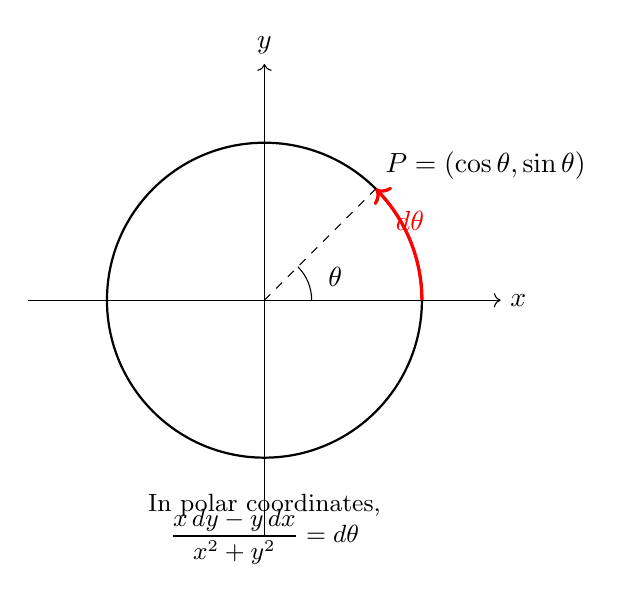
\begin{tikzpicture}[scale=2]
	% Draw coordinate axes
	\draw[->] (-1.5,0) -- (1.5,0) node[right] {$x$};
	\draw[->] (0,-1.5) -- (0,1.5) node[above] {$y$};
	
	% Draw unit circle centered at (0,0)
	\draw[thick] (0,0) circle (1);
	
	% Define an angle theta (in degrees)
	\def\thetaAngle{45}  % For example, 45 degrees
	
	% Calculate point P on the circle corresponding to theta
	\coordinate (P) at ({cos(\thetaAngle)}, {sin(\thetaAngle)});
	
	% Draw radius to point P
	\draw[dashed] (0,0) -- (P);
	\node at (P) [above right] {$P=(\cos\theta,\sin\theta)$};
	
	% Draw an arc on the circle from 0 to theta
	\draw[red, very thick, ->] (1,0) arc (0:\thetaAngle:1);
	
	% Label the arc element dtheta (placed midway along the arc)
	\node at ({cos(\thetaAngle/2)},{sin(\thetaAngle/2)}) [red, above] {$d\theta$};
	
	% Mark a small angle at the origin to indicate theta
	\draw (0.3,0) arc (0:\thetaAngle:0.3);
	\node at (0.45,0.15) {$\theta$};
	
	% Annotation showing equivalence in polar coordinates
	\node at (0,-1.3) {\small In polar coordinates,};
	\node at (0,-1.5) {\small $\displaystyle \frac{x\,dy-y\,dx}{x^2+y^2}=d\theta$};
\end{tikzpicture}

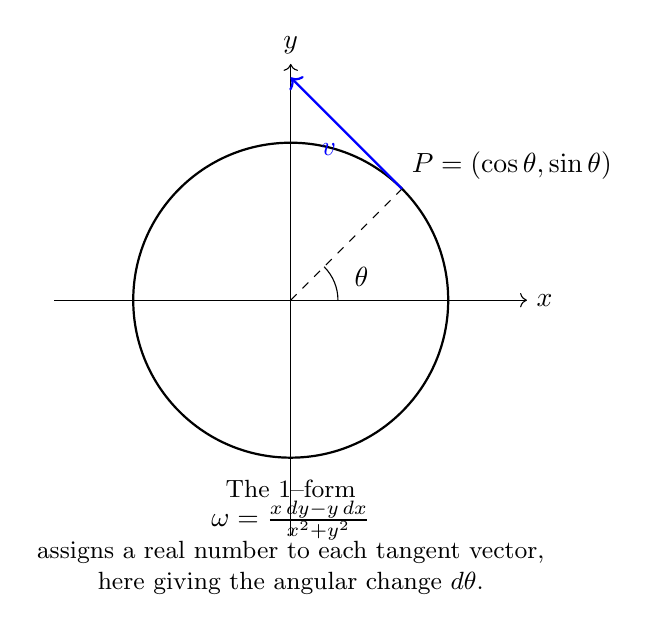
\begin{tikzpicture}[scale=2]
	% Draw coordinate axes
	\draw[->] (-1.5,0) -- (1.5,0) node[right] {$x$};
	\draw[->] (0,-1.5) -- (0,1.5) node[above] {$y$};
	
	% Draw unit circle centered at (0,0)
	\draw[thick] (0,0) circle (1);
	
	% Define an angle theta (in degrees)
	\def\thetaAngle{45}  % Example angle
	
	% Calculate point P on the circle corresponding to theta
	\coordinate (P) at ({cos(\thetaAngle)}, {sin(\thetaAngle)});
	
	% Draw radius to point P
	\draw[dashed] (0,0) -- (P);
	\node at (P) [above right] {$P=(\cos\theta,\sin\theta)$};
	
	% Draw the tangent vector at point P.
	% For a point at angle theta, a tangent vector can be represented by (-sin(theta), cos(theta))
	\draw[blue, thick,->] (P) -- ++({-sin(\thetaAngle)}, {cos(\thetaAngle)}) node[midway, below left] {$v$};
	
	% Draw a small arc near the origin to indicate the angle theta
	\draw (0.3,0) arc (0:\thetaAngle:0.3);
	\node at (0.45,0.15) {$\theta$};
	
	% Annotation explaining the 1-form concept
	\node at (0,-1.2) {\small The 1--form};
	\node at (0,-1.4) {\(\omega=\frac{x\,dy-y\,dx}{x^2+y^2}\)};
	\node at (0,-1.6) {\small assigns a real number to each tangent vector,};
	\node at (0,-1.8) {\small here giving the angular change \(d\theta\).};
\end{tikzpicture}
\newpage




%However, it is important to note that \(S^1\) itself is not a cyclic group because no single element can generate the entire uncountable set. 
%A group \(G\) is called \textbf{cyclic} if there exists an element \(g \in G\) such that
%\[
%G = \langle g \rangle = \{ g^n : n \in \mathbb{Z} \}.
%\]
%In the context of \(S^1\), while the full group is not cyclic, every finite subgroup of \(S^1\) is cyclic.
%
%\(S^1\) is a compact, connected, and smooth one-dimensional manifold. Its compactness follows from the Heine-Borel theorem, and its connectedness is inherent in the continuity of the circle. These topological features are critical in understanding its role as a topological group.
%
%Though \(S^1\) is a group under multiplication, it is not cyclic. To see this, consider any element \( e^{i\theta} \in S^1 \). The subgroup generated by \( e^{i\theta} \) is:
%\[
%\langle e^{i\theta} \rangle = \{ e^{in\theta} : n \in \mathbb{Z} \}.
%\]
%If \(\theta/2\pi\) is irrational, then \(\langle e^{i\theta} \rangle\) is dense in \(S^1\) but does not equal \(S^1\) since it is countable. If \(\theta/2\pi\) is rational, the subgroup is finite. In either case, no single element can generate the entire uncountable group \(S^1\).
%
%The exponential map provides a natural connection between the additive group \(\mathbb{R}\) and the multiplicative group \(S^1\):
%\[
%\exp: \mathbb{R} \to S^1, \quad \exp(i\theta) = e^{i\theta}.
%\]
%This continuous group homomorphism is essential in many areas of analysis and differential geometry.
%\begin{center}
%	\begin{tikzpicture}[>=stealth, scale=0.8]
%		% Real line
%		\draw[->] (-4,0) -- (4,0) node[right] {\(\mathbb{R}\)};
%		\node at (-4,0.3) {\(-\infty\)};
%		\node at (4,0.3) {\(+\infty\)};
%		
%		% S^1: Draw circle to the right
%		\begin{scope}[shift={(8,0)}]
%			\draw[thick] (0,0) circle (2cm);
%			\draw[->] (0,0) -- (2,0) node[right] {$1$};
%			\node at (0,2.3) {\(S^1\)};
%		\end{scope}
%		
%		% Arrow from real line to circle (representing the exponential map)
%		\draw[->, thick] (2,0.5) -- (7,1.5) node[midway, above] {\(\exp(i\theta)\)};
%	\end{tikzpicture}
%\end{center}
%For any positive integer \(n\), the \(n\)th roots of unity form a finite cyclic subgroup of \(S^1\). Specifically, define:
%\[
%C_n = \{ e^{2\pi i k/n} : k = 0, 1, \dots, n-1 \}.
%\]
%This group is cyclic because it can be generated by the element:
%\[
%e^{2\pi i/n},
%\]
%and every element in \(C_n\) is a power of this generator.
%
%The cyclic group \(C_n\) is a fundamental object in various fields:
%\begin{itemize}
%	\item \textbf{Number Theory:} The \(n\)th roots of unity are closely related to cyclotomic polynomials.
%	\item \textbf{Signal Processing:} They appear in the discrete Fourier transform (DFT).
%	\item \textbf{Algebra:} Finite cyclic groups are among the simplest groups and serve as building blocks for more complex structures.
%\end{itemize}
%
%\(S^1\) is not only a topological group but also a Lie group. Its smooth manifold structure enables the study of continuous group representations and provides a gateway into harmonic analysis.
%
%The study of \(S^1\) and its subgroups extends to many areas:
%\begin{itemize}
%	\item \textbf{Differential Geometry:} \(S^1\) serves as an example of a smooth manifold with a rich geometric structure.
%	\item \textbf{Complex Analysis:} As the boundary of the unit disk, \(S^1\) plays a key role in conformal mappings and function theory.
%	\item \textbf{Algebraic Topology:} The fundamental group of \(S^1\) is isomorphic to \(\mathbb{Z}\), providing insight into covering spaces and homotopy theory.
%\end{itemize}
%
%Recall that a group \(G\) is called \emph{cyclic} if
%\[
%\exists\, a \in G\;\text{s.t.}\; \forall\, g \in G,\; \exists\, n \in \mathbb{Z}:\; g = a^n.
%\]
%Consider the circle
%\[
%S^1 \coloneqq \{\, z \in \mathbb{C} \mid |z|=1 \,\},
%\]
%which is a group under complex multiplication. Each element of \(S^1\) may be written in the form
%\[
%z = e^{2\pi i \theta}, \quad \theta \in [0,1),
%\]
%and for a fixed irrational \(\theta_0\), the subgroup
%\[
%\langle e^{2\pi i \theta_0} \rangle = \{\, e^{2\pi i n \theta_0} \mid n \in \mathbb{Z} \,\}
%\]
%is dense in \(S^1\). In the finite setting, for any \(n\in\mathbb{N}\), the subgroup of \(n\)th roots of unity
%\[
%\mu_n = \{\, e^{2\pi i k/n} \mid k=0,1,\dots,n-1 \,\}
%\]
%is cyclic, isomorphic to \(\mathbb{Z}/n\mathbb{Z}\).
%\begin{tikzpicture}[scale=3]
%	
%	% Draw unit circle and axes
%	\draw[thick] (0,0) circle (1);
%	\draw[->] (-1.2,0) -- (1.2,0) node[right] {$\Re(z)$};
%	\draw[->] (0,-1.2) -- (0,1.2) node[above] {$\Im(z)$};
%	
%	% Axis labels
%	\node[below right] at (1,0) {$1$};
%	\node[below left]  at (-1,0) {$-1$};
%	\node[above left]  at (0,1) {$i$};
%	\node[below left]  at (0,-1) {$-i$};
%	
%	% Roots of unity: mu_7
%	\foreach \k in {0,...,6} {
%		\coordinate (mu\k) at ({cos(360/7*\k)},{sin(360/7*\k)});
%		\filldraw[blue] (mu\k) circle (0.015);
%	}
%	
%	% Connect cyclically: safer version without 'evaluate'
%	\foreach \k in {0,...,6} {
%		\pgfmathsetmacro{\next}{mod(\k+1,7)}
%		\draw[blue!50, thick, ->] (mu\k) -- (mu\next);
%	}
%	
%	% Label for mu_7
%	\node[blue!70!black] at (0.65,0.5) {$\mu_7 \cong \mathbb{Z}/7\mathbb{Z}$};
%	
%	% Dense subgroup: simulate e^{2\pi i n theta_0} for irrational theta_0
%	% Precomputed mod(n*0.4142,1)*360 degrees for n=1..40
%	\foreach \angle in {
%		149.1, 298.3, 87.4, 236.6, 25.7, 174.9, 324.0,
%		113.2, 262.3, 51.5, 200.6, 349.8, 138.9, 288.1,
%		77.2, 226.4, 15.5, 164.7, 313.8, 103.0, 252.1,
%		41.3, 190.4, 339.6, 128.7, 277.9, 67.0, 216.2,
%		5.3, 154.5, 303.6, 92.8, 241.9, 31.1, 180.2,
%		329.4, 118.5, 267.7, 56.8, 206.0
%	}{
%		\fill[red] ({cos(\angle)}, {sin(\angle)}) circle (0.008);
%	}
%	
%	% Labels
%	\node[red!80!black, below left] at (-0.9,-0.9) 
%	{$\langle e^{2\pi i \theta_0} \rangle$ (dense)};
%	\node at (0,-1.4) {$S^1 = \{\, z \in \mathbb{C} \mid |z|=1 \,\}$};
%	
%\end{tikzpicture}

\newpage
\section{Torus}
\begin{center}
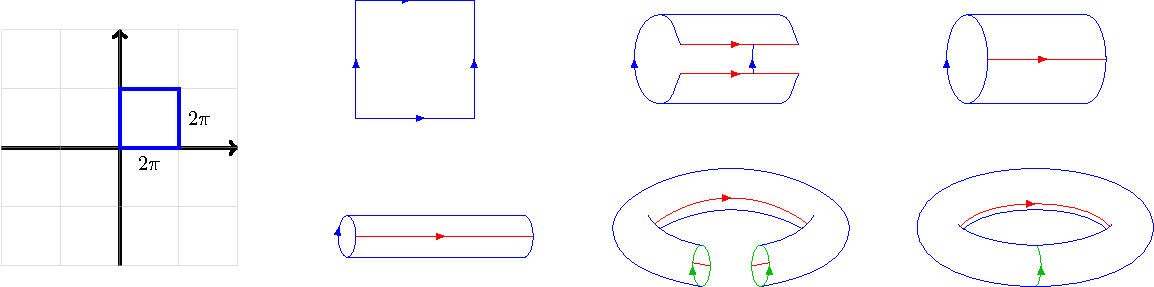
\includegraphics[scale=.85]{../tikz/grad-math-tikz-algebra/torus.pdf}
\end{center}
Consider the Cartesian product \(\mathbb{R}^2\) and the subgroup \(\mathbb{Z}^2 \subset \mathbb{R}^2\), where
\[
\mathbb{Z}^2 = \{(m,n) \mid m,n \in \mathbb{Z}\}.
\]
The quotient space is defined by the equivalence relation on \(\mathbb{R}^2\)
\[
(x,y) \sim (x',y') \quad \Longleftrightarrow \quad (x-x',y-y') \in \mathbb{Z}^2.
\]
Denote the quotient by
\[
T^2 := \mathbb{R}^2/\mathbb{Z}^2.
\]

We claim that there exists a natural homeomorphism
\[
\Phi: \mathbb{R}^2/\mathbb{Z}^2 \to (\mathbb{R}/\mathbb{Z}) \times (\mathbb{R}/\mathbb{Z}).
\]
Define the map
\[
\Phi\big((x,y)+\mathbb{Z}^2\big) = \big(x+\mathbb{Z},\, y+\mathbb{Z}\big).
\]
This mapping is well-defined because if \((x,y)\) and \((x',y')\) represent the same equivalence class, then \((x-x',y-y') \in \mathbb{Z}^2\) and hence \(x+\mathbb{Z} = x'+\mathbb{Z}\) and \(y+\mathbb{Z} = y'+\mathbb{Z}\). Moreover, \(\Phi\) is bijective and continuous with continuous inverse. 

Since we have already established that \(\mathbb{R}/\mathbb{Z} \cong S^1\) (via the homeomorphism \(\varphi\)), it follows that
\[
(\mathbb{R}/\mathbb{Z}) \times (\mathbb{R}/\mathbb{Z}) \cong S^1 \times S^1.
\]
By definition, the torus is the topological space
\[
T^2 \equiv S^1 \times S^1.
\]
Thus, we conclude that
\[
\mathbb{R}^2/\mathbb{Z}^2 \cong S^1 \times S^1,
\]
which shows that \(\mathbb{R}^2/\mathbb{Z}^2\) is, indeed, a torus.

Summary in Symbolic Notation

1. Let
\[
\mathbb{R}/\mathbb{Z} \overset{\varphi}{\cong} S^1, \quad \varphi(x+\mathbb{Z}) = e^{2\pi i x}.
\]
2. Define the quotient
\[
T^2 = \mathbb{R}^2/\mathbb{Z}^2, \quad (x,y) \sim (x',y') \iff (x-x',y-y') \in \mathbb{Z}^2.
\]
3. Then the canonical isomorphism
\[
\Phi: \mathbb{R}^2/\mathbb{Z}^2 \to (\mathbb{R}/\mathbb{Z}) \times (\mathbb{R}/\mathbb{Z}),\quad \Phi((x,y)+\mathbb{Z}^2) = (x+\mathbb{Z},\, y+\mathbb{Z})
\]
implies
\[
\mathbb{R}^2/\mathbb{Z}^2 \cong S^1 \times S^1,
\]
and hence, \(T^2\) is topologically a torus.

This completes the formal demonstration that \(\mathbb{R}^2/\mathbb{Z}^2\) is a torus.

\newpage
From the perspective of algebraic geometry—what you refer to as "zariskitology"—it is indeed more natural and fruitful to work with complex tori rather than real tori. Here’s why:

1. Enhanced Structure of \(\mathbb{C}\) vs. \(\mathbb{R}^2\)

- **Complex Field \(\mathbb{C}\):**  
The field \(\mathbb{C}\) carries a richer structure than \(\mathbb{R}^2\) when viewed as a real vector space. In particular, \(\mathbb{C}\) is not only a two-dimensional real vector space but also a one-dimensional complex vector space. This extra algebraic structure permits the definition of holomorphic functions and endows the quotient \(\mathbb{C}/\Lambda\) with the structure of a complex manifold.

- **Real Quotient \(\mathbb{R}^2/\mathbb{Z}^2\):**  
Although \(\mathbb{R}^2/\mathbb{Z}^2\) is homeomorphic to the torus \(S^1 \times S^1\) in the Euclidean (or metric) topology, it does not naturally carry a complex structure. Thus, from an algebraic-geometric point of view, the analytic and algebraic tools available over \(\mathbb{C}\) are not directly applicable.

2. Complex Tori and Elliptic Curves

- **Definition of a Complex Torus:**  
Let \(\Lambda \subset \mathbb{C}\) be a lattice, i.e.,
\[
\Lambda = \{ \omega_1 m + \omega_2 n \mid m, n \in \mathbb{Z} \},
\]
where \(\omega_1, \omega_2 \in \mathbb{C}\) are \(\mathbb{R}\)-linearly independent. Then the quotient
\[
E = \mathbb{C}/\Lambda
\]
is a complex torus. It naturally inherits the structure of a compact Riemann surface of genus one.

- **Algebraic Structure:**  
A fundamental result in complex algebraic geometry states that every complex torus of dimension one is isomorphic (as a complex analytic manifold) to an elliptic curve, i.e., a smooth projective algebraic curve of genus one. This identification allows one to apply tools from the theory of elliptic functions, modular forms, and scheme theory.

- **Zariski Topology:**  
In algebraic geometry, the Zariski topology on an algebraic variety is defined in terms of polynomial equations. The coordinate rings and the associated structure sheaves are far more natural when working over \(\mathbb{C}\) than over \(\mathbb{R}\), because algebraically closed fields like \(\mathbb{C}\) yield a richer theory (e.g., every non-constant polynomial over \(\mathbb{C}\) has a root).

3. Summary and Conclusion

Replacing \(\mathbb{R}^2\) with \(\mathbb{C}\) in the quotient construction shifts the setting from a purely topological or metric one (as in \(\mathbb{R}^2/\mathbb{Z}^2\)) to one with both complex analytic and algebraic structure. Concretely, the quotient

\[
\mathbb{C}/\Lambda,
\]

where \(\Lambda\) is a lattice in \(\mathbb{C}\), is not only a topological torus but also a complex manifold and, by the theory of elliptic curves, an algebraic curve. This richer structure is essential in algebraic geometry and offers deeper insights and more powerful tools than what the real quotient \(\mathbb{R}^2/\mathbb{Z}^2\) provides.

Thus, from a "zariskitology" (algebraic geometry) perspective, it is indeed better and more natural to consider complex tori \(\mathbb{C}/\Lambda\) rather than real tori \(\mathbb{R}^2/\mathbb{Z}^2\).

%\begin{center}
%\tdplotsetmaincoords{70}{110}
%\begin{tikzpicture}[tdplot_main_coords, scale=3]
%	
%	% Define the major and minor radii of the torus
%	\def\R{2} % Major radius (distance from the center of the torus to the center of the tube)
%	\def\r{0.5} % Minor radius (radius of the tube)
%	
%	% Draw curves of constant phi (circles around the tube)
%	\foreach \phi in {0,15,...,345} {
%		\draw[domain=0:360, smooth, variable=\theta, green!75!black, opacity=0.5]
%		plot ({(\R+\r*cos(\theta))*cos(\phi)},{(\R+\r*cos(\theta))*sin(\phi)},{\r*sin(\theta)});
%	}
%	
%	% Draw curves of constant theta (circles along the torus body)
%	\foreach \theta in {0,15,...,345} {
%		\draw[domain=0:360, smooth, variable=\phi, red, opacity=0.5]
%		plot ({(\R+\r*cos(\theta))*cos(\phi)},{(\R+\r*cos(\theta))*sin(\phi)},{\r*sin(\theta)});
%	}
%	% Optionally, label the axes
%%	\draw[->] (0,0,0) -- (3,0,0) node[anchor=north east] {\(x\)};
%%	\draw[->] (0,0,0) -- (0,3,0) node[anchor=north west] {\(y\)};
%%	\draw[->] (0,0,0) -- (0,0,2) node[anchor=south] {\(z\)};
%\end{tikzpicture}
%\end{center}

%The torus is defined as
%\[
%T^2 \coloneqq S^1 \times S^1.
%\]
%Since each factor \(S^1\) is a cyclic group (in both its finite and infinite manifestations), the torus inherits a structure where the two “circulating” (cyclic) directions coexist. In particular, the Lie group structure of \(T^2\) is given by the coordinatewise multiplication:
%\[
%(z_1, w_1) \cdot (z_2, w_2) = (z_1 z_2,\, w_1 w_2).
%\]
%Moreover, its fundamental group is
%\[
%\pi_1(T^2) \cong \pi_1(S^1) \times \pi_1(S^1) \cong \mathbb{Z} \times \mathbb{Z},
%\]
%which is not cyclic but contains many cyclic subgroups (e.g., the subgroup generated by \((p,q)\) with \(\gcd(p,q)=1\)).
%
%Thus, when learning about cyclic groups, one simultaneously gains insight into the structure of the torus: each factor of \(T^2\) embodies the essence of cyclicity, and the torus itself is a geometric object built from these circulating (cyclic) components.
%
%
%
%- **Learning \(S^1\):** One studies the cyclic nature of \(S^1\) through its generators (e.g., \(e^{2\pi i \theta}\)) and observes both finite (roots of unity) and infinite (dense subgroup) cyclic behaviors.
%
%
%- **Understanding \(T^2\):** The torus \(T^2\) is then naturally introduced as the Cartesian product \(S^1 \times S^1\), making the connection explicit: the torus is built from two copies of the cyclic group \(S^1\).
%- **Visualization:** The TikZ diagram visually encapsulates this dual structure, reinforcing that the cyclic groups are the “circulating” components whose product yields the torus.
%
%This integrated approach allows one to simultaneously appreciate the algebraic simplicity of cyclic groups and their geometric realization in the topology of the torus.
%
%\newpage
%Now consider the unit square in the complex plane: from \(0\) to \(1+i\). This forms a fundamental domain for the complex lattice \(\mathbb{Z} + i\mathbb{Z}\), relevant in the study of complex tori and elliptic curves.
%
%\subsection*{Elliptic Curve over \(\mathbb{C}\)}
%
%We now consider the set:
%\[
%E = \left\{ (x,y) \in \mathbb{C}^2 \,\middle|\, y^2 = 4x^3 + 4x \right\}
%\]
%This defines a **complex elliptic curve**, smooth and projective.
%
%\subsection*{Holomorphic Mapping}
%Let \( z \in \mathbb{C} \), and define:
%\[
%z \mapsto (\varphi(z), \varphi'(z))
%\]
%where \( \varphi \) is a suitable elliptic function (e.g., Weierstrass \(\wp(z)\)) satisfying:
%\[
%(\varphi')^2 = 4\varphi^3 + 4\varphi
%\]
%so that the image lies on \( E \).
%
%\begin{center}
%	\begin{tikzpicture}[scale=2.5]
%		
%		% Draw complex plane grid
%		\fill[blue!10,opacity=0.2] (0,0) rectangle (1,1);
%		\draw[step=0.2,gray!50,very thin] (0,0) grid (1.2,1.2);
%		\draw[thick, blue] (0,0) rectangle (1,1);
%		\node at (1.1,1.05) {\(1+i\)};
%		\node at (-0.1,0) {\(0\)};
%		\node at (1.05,0) {\(1\)};
%		\node at (0,1.05) {\(i\)};
%		\node[blue!70!black] at (0.5, -0.2) {\textbf{Fundamental domain in } \(\mathbb{C}\)};
%		
%		% Arrow to curve
%		\draw[->, thick] (1.5,0.5) -- (2.8,0.5) node[midway,above] 
%		{\( z \mapsto (\varphi(z), \varphi'(z)) \)};
%		
%		% Elliptic curve symbolically
%		\begin{scope}[xshift=3.2cm]
%			\draw[domain=-1.2:1.2, smooth, variable=\x, thick, red]
%			plot ({\x}, {\x*\x*\x + \x});
%			\node at (0,-0.5) {\( y^2 = 4x^3 + 4x \)};
%		\end{scope}
%		
%	\end{tikzpicture}
%\end{center}
%\section*{Conclusion}
%
%This sequence of mappings:
%\[
%t \mapsto (\cos t, \sin t) \quad \leadsto \quad z \mapsto (\varphi(z), \varphi'(z))
%\]
%demonstrates a path from elementary trigonometry to deep connections in algebraic and complex geometry — culminating in the geometry of elliptic curves over \(\mathbb{C}\).


\end{document}
